\documentclass[a4paper,12pt]{article}

\usepackage[left=2cm,right=2cm,top=2cm,bottom=2cm]{geometry}
\usepackage{setspace}
\onehalfspacing

\usepackage{polyglossia}
\setdefaultlanguage[babelshorthands=true]{russian}
\setotherlanguage{english}

\usepackage{fontspec}
\setmainfont{FreeSerif}
\newfontfamily{\russianfonttt}[Scale=0.7]{DejaVuSansMono}

\usepackage[tiny, compact]{titlesec}

\usepackage{titling}
\setlength{\droptitle}{-1cm}
\pretitle{\begin{center}\begin{bfseries}\Large}
\posttitle{\par\end{bfseries}\end{center}}
\preauthor{\begin{center}\normalsize}
\postauthor{\par\end{center}\vspace{-1.8cm}}

\usepackage{hyperref}
\usepackage{bookmark}
\usepackage{csquotes}
\usepackage{enumitem}
\usepackage{graphicx}
\usepackage{amsmath}
\usepackage{xcolor}
\usepackage{booktabs}
\usepackage{listings}

\lstdefinelanguage{FSharp}{
    morekeywords={let, new, match, with, rec, open, module, namespace, type, of, member, and, for, in, do, begin, end, fun, function, return, yield, try, mutable, if, then, else, elif, array, seq, list, return!, val},
    keywordstyle=\color{blue}\bfseries,
    ndkeywords={Empty, Node, Ok, Error, Result, Tree, AVLSet, ParallelAVLSet},
    ndkeywordstyle=\color{teal}\bfseries,
    identifierstyle=\color{black},
    sensitive=true,
    morecomment=[l]{//},
    morecomment=[s]{(*}{*)},
    commentstyle=\color{gray}\ttfamily,
    stringstyle=\color{red}\ttfamily,
    morestring=[b]",
    morestring=[b]"""
}
\lstset{
    language=FSharp,
    basicstyle=\small\ttfamily,
    breaklines=true,
    frame=single,
    numbers=left,
    numberstyle=\tiny\color{gray},
    xleftmargin=15pt,
    showstringspaces=false,
    captionpos=b
}

\title{Реализация типа \enquote{Множество} на основе АВЛ-дерева на языке F\#}
\author{Тарануха Леонид Антонович}
\date{}

\begin{document}

\maketitle

\begin{flushright}
\begin{tabular}{r}
    Группа: \emph{\enquote{25.Б73-мм}} \\
    Кафедра: \emph{системного программирования} \\
    Научный руководитель: \emph{Григорьев Семен Вячеславович} \\
    Номер семестра практики: \emph{2} \\
\end{tabular}
\end{flushright}

\section{Постановка задачи}

Данная работа посвящена реализации неизменяемой структуры данных \enquote{Множество} на основе АВЛ-дерева на языке F\#. Проект выполняется в рамках сообщества Lamagraph. LamaGraph~--- это проект по разработке специализированного вычислителя для разреженной линейной алгебры и специализированного языка программирования для него. Разработка вычислителя включает в себя прототипирование различных его частей и подсистем. Разработка языка заключается не только в создании его синтаксиса и транслятора, но также в разработке и прототипировании частей среды выполнения и пользовательских библиотек. Данная структура интегрируется в репозиторий QTreeFSharp.

Фундаментальные алгоритмы анализа графов требуют эффективных структур для хранения уникальных элементов и выполнения теоретико-множественных операций.

\textbf{Целью работы является} реализация структуры данных \enquote{Множество} с автоматической балансировкой АВЛ-дерева, на основе которого она написана, и оценка ее производительности.

Для достижения поставленной цели были сформулированы следующие \textbf{задачи}.
\begin{itemize}
    \item Реализовать структуру АВЛ-дерева и базовые операции (добавление, удаление, поиск).
    \item Реализовать теоретико-множественные операции (\verb|union|, \verb|intersection|, \verb|difference|, \verb|symmDifference|).
    \item Разработать альтернативные последовательному подходы к выполнению операций: на основе рекурсивного обхода и многопоточности.
    \item Написать модульные (Unit) и property-based тесты.
    \item Провести тестирование производительности разработанных алгоритмов с использованием BenchmarkDotNet.
\end{itemize}

\section{Описание предлагаемого решения}

Тип \verb|AVLSet<'Value>| представляет собой неизменяемое АВЛ-дерево. Как показано в листинге~\ref{lst:base_types}, узел дерева содержит высоту, значение и ссылки на левое и правое поддеревья. Для обработки возможных ошибок, связанных с нарушением инвариантов дерева (например, некорректная высота узла), используется монада \verb|Result| и специальный тип ошибок \verb|AVLSetError| вместо исключений.

\begin{lstlisting}[caption={Определение базовых типов}, label={lst:base_types}]
type AVLSet<'Value> =
    | Empty
    | Node of int * 'Value * AVLSet<'Value> * AVLSet<'Value>

type AVLSetError =
    | RotationError
    | InvalidHeightOfNode
    | EmptyNodeWasNotExpected
\end{lstlisting}

Балансировка осуществляется стандартными алгоритмами малых и больших вращений (\verb|LLrotate|, \verb|RRrotate|, \verb|LRrotate|, \verb|RLrotate|). 

Реализовано три подхода к операциям над множествами.

\begin{enumerate}
    \item \textbf{Последовательный.} Базовый алгоритм рекурсивного слияния. Использует функции \verb|split| (разделение дерева по ключу) и \verb|join| (слияние). Является эталоном производительности.
    
    \item \textbf{Оптимизация обходом.} Алгоритм для множеств со значительной разницей в размерах. Выполняет обход элементов меньшего множества с применением соответствующих операций к большему множеству с помощью функции \verb|traverseRes|.

    \item \textbf{Параллельный.} Многопоточная реализация, использующая \verb|Async.Parallel| для асинхронной обработки левого и правого поддеревьев после операции \verb|split|.
\end{enumerate}

Корректность алгоритмов и сохранение свойств АВЛ-дерева подтверждены с помощью библиотек Xunit, FsUnit и FsCheck.

\section{Эксперименты}

Тестирование производительности выполнялось с помощью библиотеки \verb|BenchmarkDotNet| (ОС Ubuntu 24.04.4 LTS). Аппаратной платформой выступал процессор 12-го поколения Intel Core i5-12450H, который располагает 1 процессорным разъемом (Socket), 8 физическими ядрами и поддерживает 8 логических потоков. Отсутствие аппаратной многопоточности (Hyper-Threading) в данной гетерогенной конфигурации обеспечивает строгую аппаратную изоляцию вычислений, что позволяет корректно оценивать накладные расходы пула потоков при параллельной обработке данных без скрытых планировщиком артефактов. В качестве среды выполнения использовалась платформа .NET SDK 10.0.109 с X64 RyuJIT. Размер базового множества $A$ и вторичного множества $B$ варьировался для оценки производительности алгоритмов при различных масштабах данных. 

В таблице~\ref{tab:summary} и на рисунках~\ref{fig:perf_log} и~\ref{fig:par_scaling} приведены ключевые результаты замеров, демонстрирующие зависимость производительности от разных входных данных и выбранного подхода.

\begin{table}[h!]
\centering
\caption{Результаты тестирования производительности (выборка)}
\label{tab:summary}

\resizebox{\textwidth}{!}{%
\begin{tabular}{lllrrl}
\toprule
\textbf{Операция} & \textbf{Размеры ($A \times B$)} & \textbf{Метод} &
\textbf{Время, мс} & \textbf{Память, МБ} & \textbf{Примечание} \\
\midrule
Разность & $1000 \times 100\,000$ & Последовательный &
$\approx 1.8$ & $\approx 2.3$ & Эталон \\
Разность & $1000 \times 100\,000$ & Обход &
95.5 & 129.7 & Острое замедление \\
Разность & $1000 \times 100\,000$ & Встроенный (HashFS) &
$\approx 0.82$ & 0 & Нулевая аллокация \\
\midrule
Разность & $10\,000 \times 100\,000$ & Последовательный &
19.1 & 13.8 & Эталон \\
Разность & $10\,000 \times 100\,000$ & Параллельный (2 потока) &
9.7 & 13.9 & Ускорение $\approx 2.0\times$ \\
Разность & $10\,000 \times 100\,000$ & Параллельный (4 потока) &
9.7 & 13.9 & Блокировки пула потоков \\
\bottomrule
\end{tabular}%
}
\end{table}

\begin{figure}[h!]
    \centering
    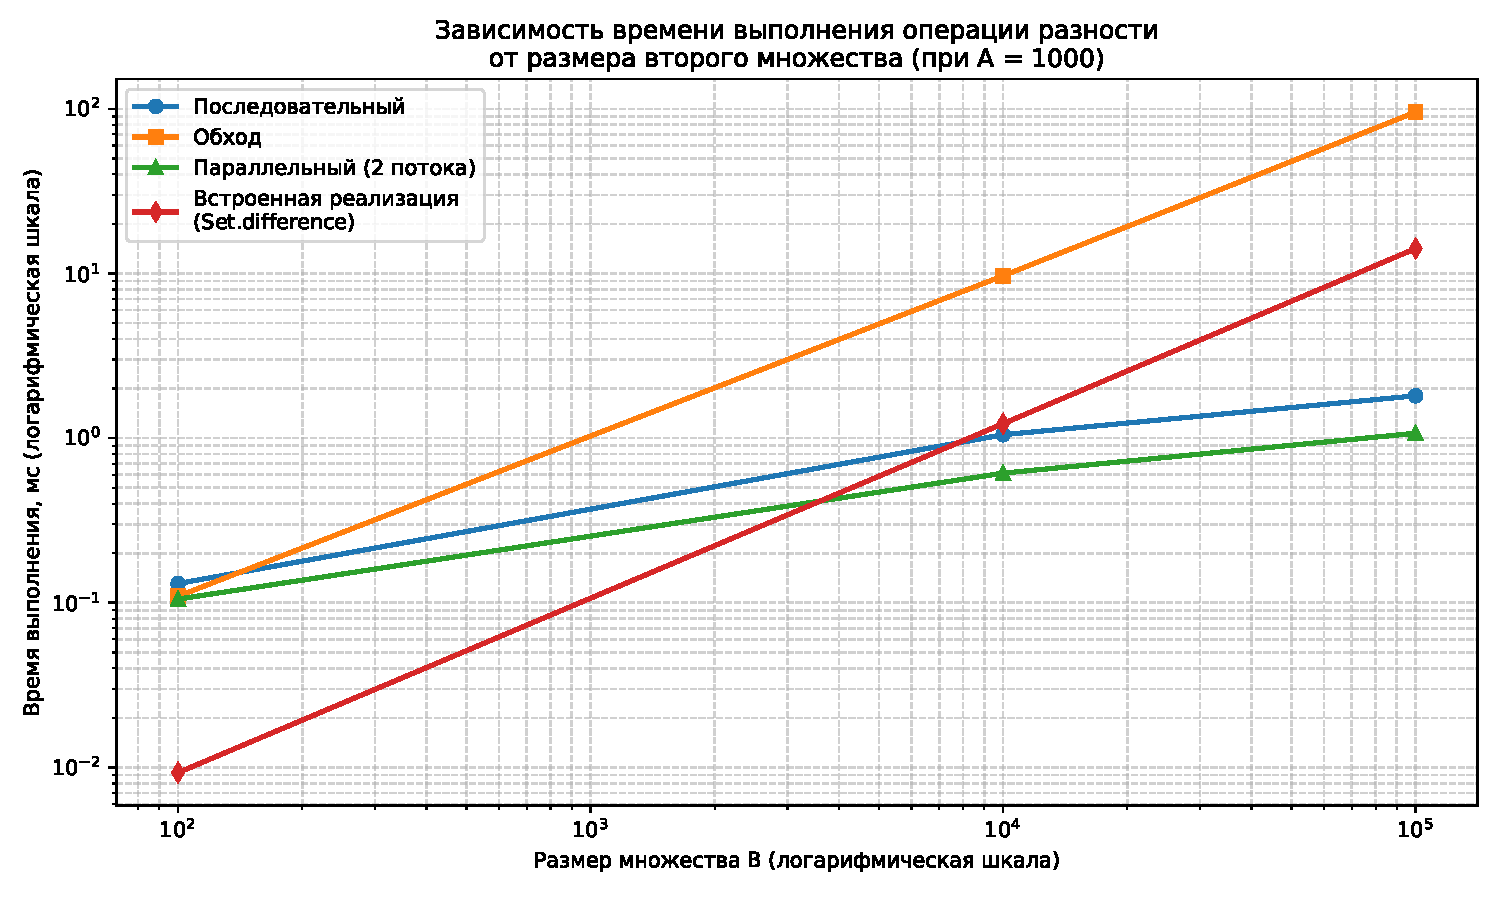
\includegraphics[width=0.9\textwidth]{images/figure1_time_log.pdf}
    \caption{Зависимость времени выполнения операции разности от размера второго множества}
    \label{fig:perf_log}
\end{figure}

\subsection{Оценка встроенных коллекций F\#}
Реализация \verb|HashSet| на всех измеренных масштабах остаётся существенно быстрее и \verb|AVLSet|, и \verb|Set|, однако её время выполнения не является постоянным: оно растёт вместе с размером второго (перебираемого) множества. Так, время операции \verb|DifferenceHashFS| держится на уровне порядка 250 нс при $B=100$ независимо от размера $A$, но возрастает до 0.82--1.31 мс при $B=100\,000$; аналогично ведёт себя \verb|UnionHashFS| (0.24 мкс при $B=100$ против 0.82--1.07 мс при $B=100\,000$), при этом аллоцируя фиксированные 40~Б на вызов независимо от размеров множеств, поскольку хэш-таблица изменяется на месте без перестроения. Даже на трудном для \verb|Set| сценарии $A=1000$, $B=100\,000$ \verb|DifferenceHashFS| (0.82 мс) опережает \verb|DifferenceFS| (14.2 мс) более чем на порядок, а по сравнению с последовательной реализацией \verb|AVLSet| (1.8 мс) преимущество сокращается примерно до 2 раз~--- поскольку время \verb|HashSet| тоже растёт вместе с $B$.

Стандартная неизменяемая реализация \verb|Set| демонстрирует сильную зависимость от соотношения размеров множеств. На наборах, где исходное множество $A$ значительно больше вычитаемого $B$ (например, $A=100\,000$, $B=100$), \verb|Set| опережает \verb|AVLSet| на операции разности (\verb|DifferenceFS| против \verb|SequentialDifferenceAVL|: 0.025 мс против 0.37 мс) и выделяет в 6.5 раза меньше памяти.

Однако на больших асимметричных наборах данных, где вычитаемое множество $B$ на порядки превосходит исходное $A$ (например, при $A=1000$, $B=100\,000$), стандартная реализация резко проигрывает: она уступает последовательной реализации почти в 8 раз по времени (14.2 мс против 1.8 мс) и выделяет в 17 раз больше памяти (39.3 МБ против 2.3 МБ).

Причина~--- в определении функции, к которой сводится оператор \verb|(-)| типа \verb|Set<'T>|: вызов \verb|A - B| выполняется как \verb|SetTree.diff set1.Comparer set1.Tree set2.Tree|, где уменьшаемое~--- \verb|set1|~=~$A$, а вычитаемое~--- \verb|set2|~=~$B$ (репозиторий dotnet/fsharp, файл \verb|FSharp.Core/set.fs|, оператор (-)~--- строка 888: \url{https://github.com/dotnet/fsharp/blob/main/src/FSharp.Core/set.fs#L888-L894}); сама функция определена как \verb|diff comparer a b = diffAux comparer b a| (там же, функция \verb|diffAux|~--- строка 372, функция \verb|diff|~--- строка 383: \url{https://github.com/dotnet/fsharp/blob/main/src/FSharp.Core/set.fs#L372-L384}). Вспомогательная \verb|diffAux| рекурсивно обходит \emph{всё} дерево своего первого аргумента~--- здесь это \verb|b|, то есть вычитаемое множество $B$,~--- и для каждого встреченного значения вызывает \verb|remove| над вторым аргументом-накопителем, изначально равным \verb|a| (то есть $A$); обход прекращается досрочно только тогда, когда накопитель становится пустым. Таким образом, число вызовов \verb|remove| равно числу узлов дерева $B$ и практически не зависит от размера $A$.

В последовательной реализации \verb|AVLSet.difference|, напротив, число вызовов \verb|Tree.split| равно числу узлов дерева $A$, а не $B$: рекурсия строится по структуре уменьшаемого множества, и на каждом его узле \verb|split| спускается лишь по одному пути от корня дерева $B$ к искомому ключу, не затрагивая остальные его узлы. Поэтому объём работы последовательной реализации растёт вместе с размером $A$, а встроенной функции~--- вместе с размером $B$; этим и объясняется наблюдаемая асимметрия при $A=1000,\,B=100\,000$.

Данная асимметрия не распространяется на объединение и пересечение. Функция \verb|SetTree.union| строится на разбиении (\verb|split|) меньшего по высоте дерева относительно корня большего~--- по тому же принципу \enquote{split/join}, что и \verb|AVLSet.union|,~--- и на измеренных данных не проигрывает ей: при $A=1000$, $B=100\,000$ \verb|UnionFS| выполняется быстрее \verb|SequentialUnionAVL| (0.50 мс против 4.86 мс) и выделяет меньше памяти (0.62 МБ против 3.62 МБ). Функция \verb|SetTree.intersection| обходит дерево первого аргумента, проверяя принадлежность каждого элемента второму множеству; при том же соотношении размеров \verb|IntersectionFS| также опережает \verb|SequentialIntersectionAVL| (0.074 мс против 2.38 мс). Рост стоимости при $B \gg A$, таким образом, характерен именно для разности, а не для объединения и пересечения.

Большое выделение памяти во всех реализациях теоретико-множественных операций для \verb|AVLSet| также объясняется тем, что код написан с использованием монады Result, поэтому на каждом вызове рекурсивных функций для теоретико-множественных операций узел \verb|AVLSet<'Value>| обернут в тип \verb|Result<'T, 'TError>|, что на вызовах с большими размером множеств выделяет еще больше памяти и нагружает сборщик мусора.

\subsection{Оценка реализации, основанной на обходе дерева}
На графике (рис. \ref{fig:perf_log}) наглядно отражено экспоненциальное возрастание времени работы алгоритма прямого обхода (\verb|DifferenceViaTreeTraversalAVL|) при увеличении размера вычитаемого множества. Алгоритм оказался крайне чувствителен к дисбалансу размеров множеств. В сценариях, где вычитаемое множество $B$ превышает исходное $A$ на два порядка (например, $1\,000$ и $100\,000$), происходит экстремальное падение производительности. 

Операция разности занимает 95.5 мс (более чем в 50 раз медленнее базового последовательного метода) и аллоцирует 129.7 МБ памяти. Это вызывает интенсивную работу сборщика мусора всех поколений и делает данный подход абсолютно непригодным для сильно асимметричных множеств.

\begin{figure}[h!]
    \centering
    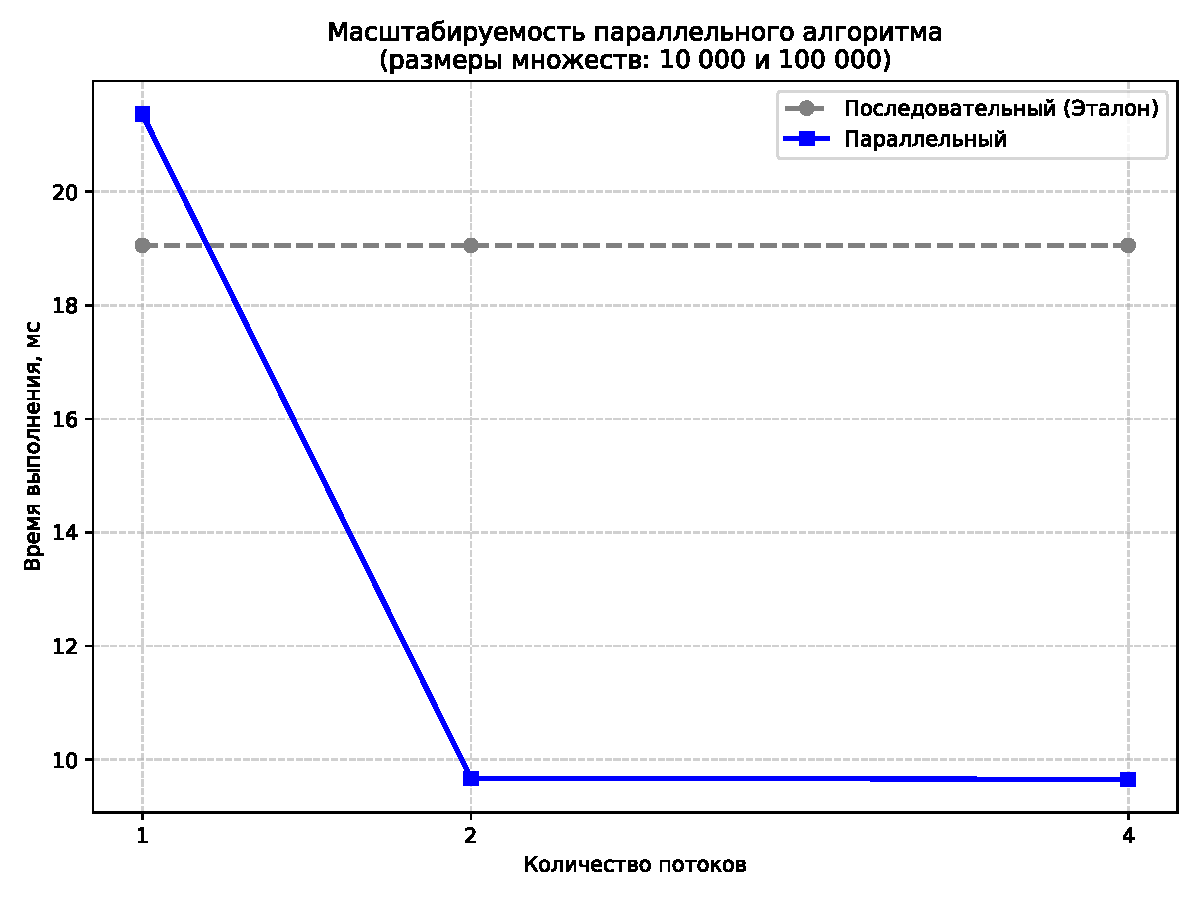
\includegraphics[width=0.8\textwidth]{images/figure2_parallel_scaling.pdf}
    \caption{Масштабируемость параллельного алгоритма (размеры $10\,000 \times 100\,000$)}
    \label{fig:par_scaling}
\end{figure}

\subsection{Оценка многопоточной реализации}
Замеры выполнялись на устройстве с 8 логическими потоками. Для оценки данной реализации параллельным функциям передавалось ограничение на 1, 2 и 4 потока. 

Как показано на графике (рис. \ref{fig:par_scaling}), распараллеливание операций (\verb|ParallelDifferenceWithThreadsAVL|) целесообразно исключительно для больших объемов данных. 

На малых наборах (например, $A=1000$, $B=100$) и при конфигурации в 1 поток параллельный алгоритм на 30\% медленнее последовательного из-за существенных затрат на маршрутизацию пула потоков. Использование 2 потоков на больших коллекциях ($10\,000 \times 100\,000$) позволяет снизить время выполнения с 19.1 мс до 9.7 мс. 

Однако масштабирование оказалось нелинейным: увеличение до 4 потоков практически не дает прироста производительности (9.7 мс). Алгоритм упирается в архитектурные ограничения и возросшее количество блокировок пула потоков.

\section{Заключение}

В ходе работы выполнены следующие задачи.
\begin{itemize}
    \item Реализована структура данных АВЛ-множества на языке F\#.
    \item Разработаны алгоритмы теоретико-множественных операций в трех вариантах (последовательный, обход, многопоточный).
    \item Написаны модульные (Unit) и property-based тесты.
    \item Проведено тестирование производительности, на основе которого выявлены условия применимости параллельного метода и метода обхода дерева.
\end{itemize}

С учетом проведенного анализа результатов тестирования производительности были сделаны следующие практические выводы.
\begin{itemize}
    \item \textbf{Последовательный алгоритм (\texttt{split}/\texttt{join})} рекомендуется в качестве метода по умолчанию. Он продемонстрировал высокую универсальность и алгоритмическую устойчивость. В условиях сильной асимметрии данных (когда вычитаемое множество на порядки больше уменьшаемого) он превосходит встроенную операцию разности \verb|Set.difference| из стандартной библиотеки F\# как по скорости выполнения (до 8 раз), так и по эффективности работы с памятью (до 17 раз меньше аллокаций); на объединении и пересечении, где встроенные алгоритмы используют иную стратегию (\verb|split|-разбиение большего дерева и обход меньшего соответственно), такого преимущества не наблюдается.
    \item \textbf{Встроенные неизменяемые коллекции F\# (\texttt{Set})} показывают превосходную производительность на соразмерных множествах, при вычитании малого множества из большого, а также на операциях объединения и пересечения асимметричных множеств; архитектурная уязвимость к избыточным аллокациям затрагивает именно операцию разности при большом вычитаемом множестве и связана с тем, что соответствующая функция (\texttt{SetTree.diff}) обходит вычитаемое множество целиком.
    \item \textbf{Множество на основе хэш-таблиц (\texttt{HashSet})} не требует перестроения дерева при изменении и на всех измеренных масштабах остаётся существенно быстрее и \texttt{AVLSet}, и стандартного \texttt{Set}, что делает его естественным выбором для локальных высоконагруженных вычислений, не требующих сохранения истории состояний. При этом его время выполнения растёт вместе с размером второго множества, так что преимущество перед последовательной реализацией \texttt{AVLSet} на разности сокращается при больших $B$~--- с сотен раз при малом $B$ до $\approx 2$ раз при $A=1000$, $B=100\,000$.
    \item \textbf{Параллельный подход} имеет смысл ограничивать пулом в 2 потока и применять исключительно на сверхбольших коллекциях данных. Дальнейшее распараллеливание приводит к снижению производительности из-за экспоненциального роста накладных расходов на синхронизацию пула потоков.
    \item \textbf{Логика обхода дерева} непригодна для использования в качестве общего решения. Она применима лишь при строго определенных и заранее известных соотношениях размеров множеств. В неблагоприятных случаях алгоритм демонстрирует катастрофическое снижение производительности: время выполнения возрастает в десятки раз, а аномальные аллокации памяти достигают 129.7 МБ на одну операцию, что приводит к сильной перегрузке сборщика мусора.
\end{itemize}

Кодовая база и результаты тестов размещены в открытом доступе.
\begin{itemize}
    \item Репозиторий: \url{https://github.com/LeoN192/AVLSetFSharp}
    \item Pull Request: \url{https://github.com/Lamagraph/QTreeFSharp/pull/17}
\end{itemize}

\renewcommand{\refname}{Литература}
\begin{thebibliography}{99}
    \bibitem{QTree} Quad-tree based linear algebra in F\# for GraphBLAS-style graph analysis [Электронный ресурс]. URL: \url{https://github.com/Lamagraph/QTreeFSharp} (дата обращения: 13.06.2026).
    \bibitem{FsCheck} FsCheck Documentation [Электронный ресурс]. URL: \url{https://fscheck.github.io/FsCheck/} (дата обращения: 13.06.2026).
    \bibitem{BenchmarkDotNet} BenchmarkDotNet [Электронный ресурс]. URL: \url{https://benchmarkdotnet.org/} (дата обращения: 13.06.2026).
    \bibitem{FSharpCore} FSharp.Core source code, module \texttt{SetTree} (файл \texttt{set.fs}) [Электронный ресурс]. URL: \url{https://github.com/dotnet/fsharp/blob/main/src/FSharp.Core/set.fs} (дата обращения: 21.09.2026).
    \bibitem{Okasaki} Okasaki C. Purely Functional Data Structures.~--- Cambridge University Press, 1998.~--- 232 p.
\end{thebibliography}

\end{document}